%File: formatting-instruction.tex
\documentclass[letterpaper]{article}
\usepackage{aaai}
\usepackage{times}
\usepackage{helvet}
\usepackage{courier}
\usepackage{hyperref}
\usepackage{comment}
\usepackage{graphicx}
\usepackage{natbib}
\frenchspacing
\setlength{\pdfpagewidth}{8.5in}
\setlength{\pdfpageheight}{11in}
\pdfinfo{
/Title (Mobile Computing -  Indoor Localization)
/Author (Daqing Yi)}
\setcounter{secnumdepth}{0}  
 \begin{document}
% The file aaai.sty is the style file for AAAI Press 
% proceedings, working notes, and technical reports.
%
\title{Mobile Computing - Indoor Localization}
%\subtitle{CS 660 Computer Networks}

\author{Daqing Yi\\
%Brigham Young University \\
\emph{dqyi11@gmail.com}
}
\maketitle

\begin{comment}
ach student will work individually to write a short survey paper examining a focused area of networking that they are interested in. 
The goal of this paper is to demonstrate your expertise in understanding Networking as a research area and to give you additional experience conducting a literature search in a new area and presenting your ideas in writing.
Your paper should summarize the 5 or 6 most important papers on a research topic and should go well beyond the papers from class.
\end{comment}

\section{Introduction}

An \emph{Indoor positioning system} locates the objects or people in an indoor environment.
Indoor localization enables indoor navigation in shopping malls, indoor location-based advertisements, friends and family member tracking and etc.

Unlike the popularity of GPS applied in outdoor localization, the GPS signal in an indoor environment can be weak.
Usually the information used for localization includes radio waves, magnetic fields, acoustic signals or other sensory information from mobile devices.
In an indoor environment, there are a lot of factors that can influence the detected signals, e.g. moving objects and complex architecture objects.
A precise localization becomes a challenge as a result.

The localization information can be directly calculated from GPS information~\cite{Nirjon:2014:CIL:2594368.2594378}, but most common ways are using the estimated distance to anchors to locate devices, which includes WiFi~\cite{Sen:2013:AMR:2462456.2464463}~\cite{Wang:2012:NNW:2307636.2307655}~\cite{Rai:2012:ZZC:2348543.2348580}~\cite{Nandakumar:2012:CLD:2348543.2348579}, Acoustic beacon~\cite{Liu:2013:GEF:2462456.2464450}~\cite{Nandakumar:2012:CLD:2348543.2348579}.
The methods to enhance the accuracy of estimations can be categorized into
\begin{itemize}
	\item technology improvement~\cite{Nirjon:2014:CIL:2594368.2594378}~\cite{Sen:2013:AMR:2462456.2464463}~\cite{Liu:2013:GEF:2462456.2464450}, 
	\item and Bayseian inference~\cite{Wang:2012:NNW:2307636.2307655}~\cite{Nandakumar:2012:CLD:2348543.2348579}~\cite{Rai:2012:ZZC:2348543.2348580}.
\end{itemize}




\begin{comment}
GPS
\cite{Nirjon:2014:CIL:2594368.2594378} 
WiFi
\cite{Sen:2013:AMR:2462456.2464463}
Acoustic beacon
\cite{Liu:2013:GEF:2462456.2464450}

\cite{Rai:2012:ZZC:2348543.2348580}

\cite{Wang:2012:NNW:2307636.2307655}
Graphical model
\cite{Nandakumar:2012:CLD:2348543.2348579}
\end{comment}

\section{GPS assisted localization}
\label{sec:gps_local}

GPS has been applied widely into the 
Due to low signal strength and multipath effect, usually the GPS receiver does not work well in an indoor building.
The indoor signal strength can be reduced 10 to 100 times of that in outdoor.

\cite{Nirjon:2014:CIL:2594368.2594378} proposes a hardware-software approach \emph{COIN-GPS}, which is a highly-sensitivity cloud-offloaded instant GPS.
It consists of three components,
\begin{itemize}
	\item a \emph{directional antenna},
	\item a \emph{robust acquisition algorithm} and
	\item a \emph{multi-directional location estimation algorithm}.
\end{itemize}

Because of the signal noise, the peak detection in common acquisition becomes difficult.
A patch antenna array is selected in \cite{Nirjon:2014:CIL:2594368.2594378}.
The use of a \emph{directional antenna} helps reduce the noise.
The reduction of the noise enable the peak search in frequency domain in weak signal in the indoor environment.
A non-coherent integrator is also used to remove the wrong peak in the presence of noise.
Least square optimization is also introduced to eliminates the multipath effect.

In practice, because there are $ 5 $ parameters $ (X, Y, Z) $, \emph{common bias} and \emph{coarse time error}, at least $ 5 $ acquired satellites are needed to estimate the location.
As a result, the indoor location estimation might be a problem due to inadequate satellites.
Because the steering of the antenna does not change the location, two sets of satellites information at different directions could be merged so that the number of unknown could reduced.
In \cite{Nirjon:2014:CIL:2594368.2594378}, nine directions are used in the format of $ (R, S) $, in which $ R $ is main beam tilt angle along the X-axis and $ S $ is the tilt angle along the Y-axis.
The directions are $ (0, 0) $ , $ (\pm 15, 0) $, $ (\pm 30, 0) $, $ (0, \pm 15) $ and $ (0, \pm 30) $.


\section{Wifi assisted localization}

Another popular way of localization is using WiFi signal. 
Signal strength(\emph{RSSI}) is used to estimate the distance to the AP, but it is hard to discriminate between multipath reflections and the direct path.
In \cite{Nirjon:2014:CIL:2594368.2594378}, \emph{CUPID} is proposed by leveraging PHY layer information along with natural human mobility.
\begin{figure}
	\centering
	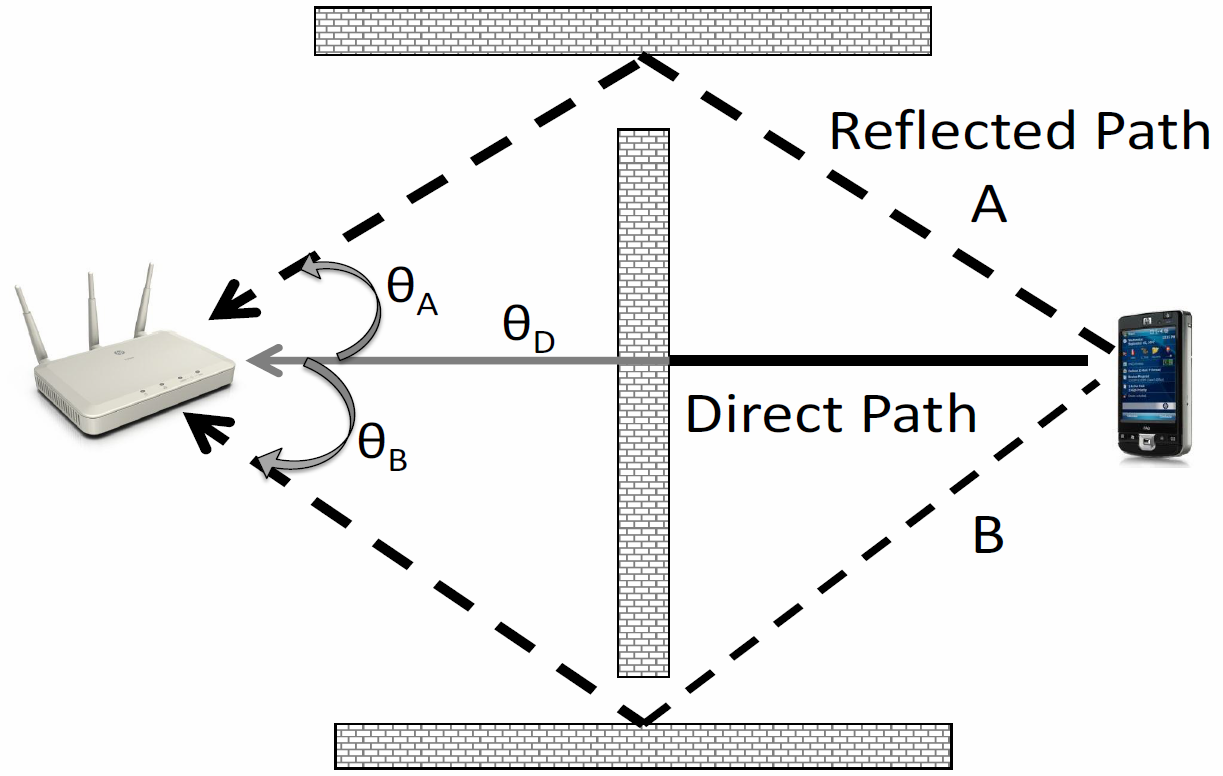
\includegraphics[width=0.7\linewidth]{fig/multipath.png}
	\caption{An example of multiple paths of wireless signal~\cite{Sen:2013:AMR:2462456.2464463}.}
	\label{fig:multipath}
\end{figure}
The localization problem becomes the estimation of the distance and the angle.
The distance estimation is obtained by \emph{EDP} (Energy of the directed path) instead of \emph{RSSI}, because it is less susceptible to mutipath reflection
\footnote{Figure \ref{fig:multipath} gives an example of multipath reflection.}.
It is extracted from \emph{CSI} (Channel state information) in the PHY layer. 
Experiments have been taken to show that this method provides a better accuracy of distance estimation than \emph{RSSI}, which the mean error is reduced from $ 10 $m to $ 4 $m.
The angle estimation is usually from \emph{AoA} (angle-of-arrival).
Usually the angle of the highest peak in MUSIC's pseudospectrum is selected as the angle of the directed path.
However, if the directed path is not blocked, the peak might correspond to a reflected path, as in Figure \ref{fig:multipath}.
The angle estimation is calculated by \emph{ANDP} (Angle of the directed path).
\begin{figure}
	\centering
	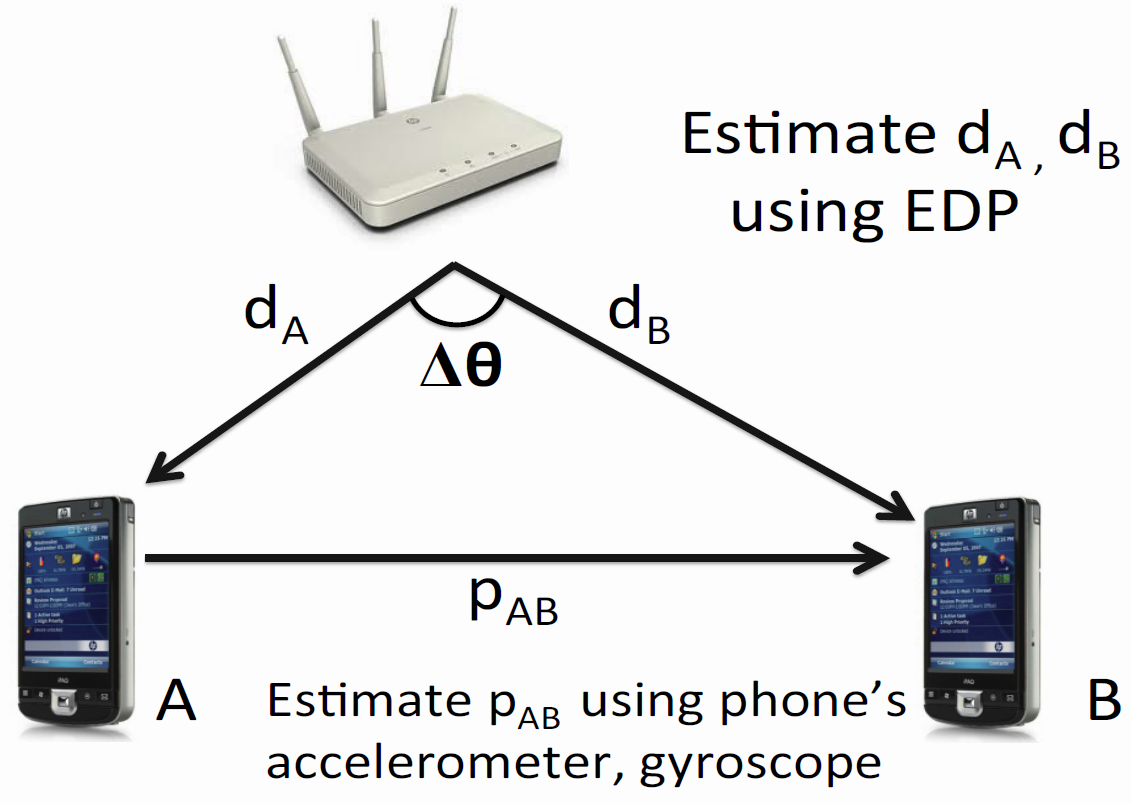
\includegraphics[width=0.7\linewidth]{fig/ANDP.png}
	\caption{Compute the change of angle using human mobility~\cite{Sen:2013:AMR:2462456.2464463}.}
	\label{fig:andp}
\end{figure}
Figure \ref{fig:andp} illustrates the calculation of
\begin{equation}
\Delta \theta = \arccos \frac{ d_{A}^{2}+d_{B}^{2}-p_{AB}^{2} }{ 2 * d_{A} * d_{B} }.
\end{equation}
The location distance $ p_{AB} $ can be obtained by the accelerometer and gyroscope of the mobile phone.

\section{Acoustic beacon assisted localization}

In \cite{Liu:2013:GEF:2462456.2464450}, an anchor network is imported for localization, which is named \emph{Guoguo}
\footnote{``Guoguo'' means Tettigonia in Chinese.}.
An anchor could transmit the spatial beacon signal to inform the unique location.
The use of acoustic communication brings
\begin{itemize}
	\item improved scalability and efficiency,
	\item and reduced hardware requirement.
\end{itemize}
\begin{figure}
	\centering
	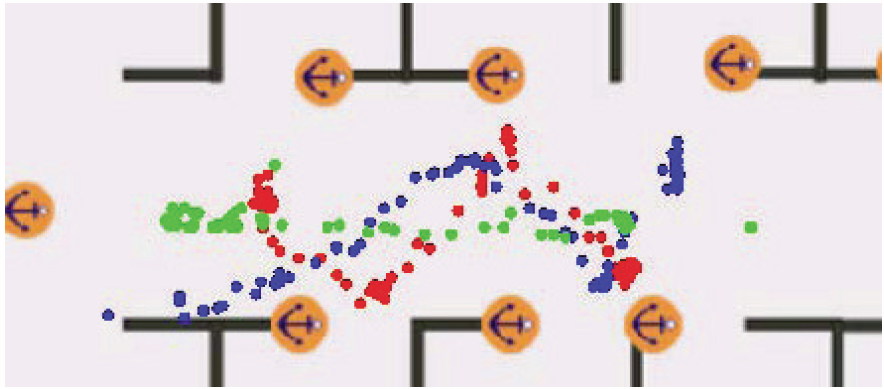
\includegraphics[width=0.9\linewidth]{fig/GUOGUO.png}
	\caption{An anchor network of Guoguo ecosystem.~\cite{Liu:2013:GEF:2462456.2464450}.}
	\label{fig:guoguo}
\end{figure}
The operation band is chosen as $ 15 kHz \sim 20 kHz $, which the human's ears are less sensitive to.
Because the beacon signal is wide-band modulated, it is unnoticeable to the humans.

In order to differentiate anchor nodes, there should be enough code distance redundancy for proper pseudo-codes.
The distance estimation depends on the TOA (Time-of-Arrival) estimation, which is performed to estimate the firsth path sample $ k^{0}_{j} $ in the whole symbol duration.
It is calculated by
\begin{equation}
\hat{k}^{0}_{j} = \min_{k} ( k \mid r_{j} (k) > \eta_{toa} ) , k \in [ k_{p} - J_{p}, K_{p} + M_{O}  ].
\end{equation}
A code matching process is called to synchronize between the anchor node and the smartphone.
After synchronization, a TOA estimation matrix $ \mathbf{r} $ can be obtained.
A sliding window of length $ W $  is applied to the TOA estimation matrix to generate a representation of current sparse measurement.
Thus the estimated distance to the anchor nodes could be updated.
All the anchor nodes are synchronized by a controller.
With the estimated distances to $ M $ anchor nodes, multilateration can be performed to localize the devices.	
By minimizing the square errors, the position could be estimated by
\begin{equation}
\hat{\theta} = (\mathbf{M}^{T} \tilde{\Sigma}^{-1} A )^{-1} A^{T} \tilde{\Sigma}^{-1} \nu.
\end{equation}


\section{Hybrid information assisted localization}

\cite{Nandakumar:2012:CLD:2348543.2348579} proposes \emph{Centaur}, a sensory information fusion for location estimation by using Bayesian inference.
The \emph{Centaur} accommodates both anchors and non-anchors.
\begin{itemize}
\item Anchors provide known locations as priori, for example an assigned desktop PC that is not likely to be moved.
\item Non-anchors are mobile devices, the locations of which need to be estimated.
\end{itemize}

The \emph{Centaur} adopts a Bayesian network of random variables.
Random variables that can be measured are labeled as evidence nodes.
Directed edges represent the relationships between the variables.
The Bayesian inference could be applied to the network structure so that the location estimation can be obtained.

In this paper, Radio Frequency (RF) and Acoustic Ranging (AR) are used for measurement.
The WiFi measurements on the locations of non-anchors are fused with geometric constraints obtained from the acoustic measurements.

Two schemes of acoustic ranging are also introduced to enhance the measurement.
\emph{EchoBeep} is introduced to make acoustic ranging more robust in non-line-of-sight setting.
It is an enhanced version of BeepBeep, an acoustic signal detection scheme.
After denoising the signals, the first received copy of the chirp signal is via the direct path (because it is the shortest), though it might be weak.
It enables reliable detection of the shortest acoustic path by additional cross-correlation processing.
\emph{DeafBeep} is proposed to adapt acoustic ranging to localize speaker-only devices, such as the desktop PCs in an office with only speakers.
It utilizes the location constraint in three devices, which is illustrated in Figure \ref{fig:deafbeep}.
\begin{figure}
	\centering
	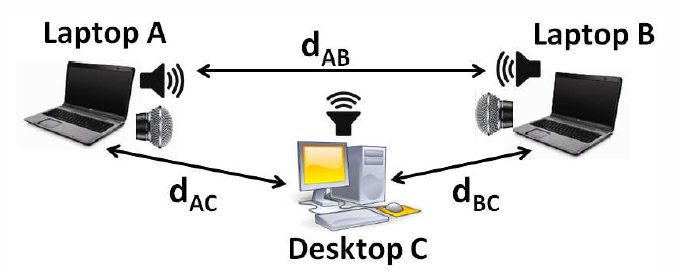
\includegraphics[width=0.7\linewidth]{fig/DeafBeep.png}
	\caption{Triangle constraint used in BeafBeep.~\cite{Nandakumar:2012:CLD:2348543.2348579}.}
	\label{fig:deafbeep}
\end{figure}

\section{Active learning based localization}

\cite{Rai:2012:ZZC:2348543.2348580} proposed \emph{Zee} as an active learning procedure for location estimation.
Instead of a labor intensive training set generation process, zero-effort crowdsourcing is reached.
\emph{Zee} performances WiFi scans and records the results indexed by time while executing the location estimation.
Each WiFi measurement is paired with an estimated location as a record of the WiFi training set.
This generated crowdsourced training dataset is fed into ``Horus'' and ``EZ'', two WiFi fingerprinting-based localization techniques.
Because the training data set is created from the walks that users take through the space of interest in normal courses.
\emph{Zee} offers a zero-effort crowdsourcing.

Two techniques are used in estimating the locations.
\begin{itemize}
\item \emph{Augmented particle filtering} is imported to represent the uncertainty in location estimation.
Moreover, it helps the tracking of latent variables, like the stride length of a user and the direction of walk.
\item \emph{Backward belief propagation} is used after the tracking has converged.
The later point in time with greater certainty could be used to reduce the uncertainty in location at earlier times.
\end{itemize}


\section{SLAM-based localization}

\cite{Wang:2012:NNW:2307636.2307655} introduced \emph{UnLoc} framework.
It simulates the SLAM (simultaneous localization and mapping) in robotics so that unsupervised localization could be reached.
The devices starts to move from a known reference location, for example, an entrance of a building.
By using dead-reckoning, the estimated location can be updated while moving.
Landmarks are also used to correct location estimation.
There are two types of landmarks.
\begin{itemize}
	\item \emph{Seed landmarks} are certain structures in the building - stairs, elevators, entrances, escalators.
	In this regions, the humans are forced to generate certain predictable behaviors.
	\item \emph{Organic landmarks} are selected from ambient signatures - in magnetic domain, WiFi signal, or even near water-fountain.
	The generation process is given in Figure \ref{fig:olm}.
	The sensed data are clustered.
	If the data in same cluster falls in a small region, an organic landmark will be created.
\end{itemize}
\begin{figure}
	\centering
	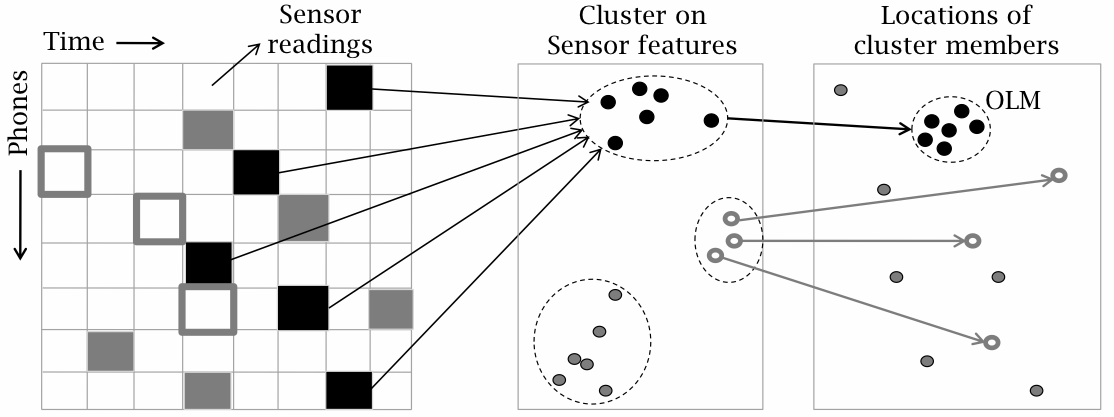
\includegraphics[width=0.9\linewidth]{fig/OLM.png}
	\caption{The generation of organic landmarks.~\cite{Wang:2012:NNW:2307636.2307655}.}
	\label{fig:olm}
\end{figure}


\section{Summary}

\begin{comment}
\begin{table}[ht]
\caption{Comparison of different methods.}
\label{tb:comparison}
\centering
\begin{center}
\begin{tabular}{|c|p{2.2cm}|p{2.2cm}|p{2.2cm}|p{2.2cm}|p{2.2cm}|p{2.2cm}|}
	\hline
	\textbf{Name} & COIN-GPS & CUPID &  Guoguo & Centaur & Zee & UnLoc \\
	\hline
	\textbf{Technology} & GPS & WiFi & AR & WiFi, AR & WiFi & Magnetic, WiFi, Accelerometer, gyroscopes \\
	\hline
	\textbf{Accuracy} & & & & & & \\         
	\hline
\end{tabular}
\end{center}
\end{table}
\end{comment}

\bibliographystyle{abbrv}
\bibliography{reference}

\end{document}
